\documentclass[e2_tp1_main.tex]{subfiles}

\begin{document}

\section{Análisis de la protección}
Se decidió utilizar una protección foldback dado que esta evita el pasarnos de la corriente de salida máxima establecida, $Io_{m\acute{a}x}=1.5\thinspace{A}$ y nos limita la cantidad de potencia a disipar por una menor a la dada por una protección lineal reduciendo costos.
Al agregar la protección foldback nos quedamos con el siguiente circuito:
\begin{figure}[H]
  \centering
   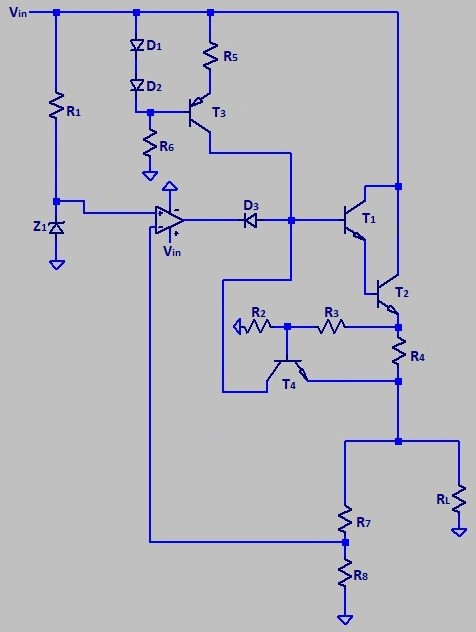
\includegraphics[width=0.5\textwidth]{CircuitoProtec.jpg}
   \caption{Circuito con protección}
   \label{fig:CircuitoProtec}
\end{figure}
De la figura ~\ref{fig:CircuitoProtec} podemos observar que la protección va a tener los siguientes parámetros:
\begin{figure}[H]
  \centering
   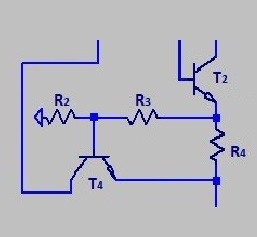
\includegraphics[width=0.5\textwidth]{AnalProtec.jpg}
   \caption{Análisis del circuito}
   \label{fig:AnalProtec}
\end{figure}
De la ~\ref{fig:AnalProtec} al recorrer la malla marcada obtenemos la siguiente ecuación:
\end{document}